\documentclass[12pt]{article}


% Math		****************************************************************************************
\usepackage{fancyhdr} 
\usepackage{amsfonts}
\usepackage{amsmath}
\usepackage{amsthm}
\usepackage{dsfont}

% Macros	****************************************************************************************
\usepackage{calc}

% Commands and Custom Variables	********************************************************************
\newcommand{\problem}[1]{\hspace{-4 ex} \large \textbf{#1}\\}
\let\oldemptyset\emptyset
\let\emptyset\varnothing

%page		****************************************************************************************
\usepackage[margin=1in]{geometry}
\usepackage{setspace}
%\doublespacing
\allowdisplaybreaks
\pagestyle{fancy}
\fancyhf{}
\rhead{Shaw \space \thepage}
\setlength\parindent{0pt}

%Code		****************************************************************************************
\usepackage{listings}
\usepackage{courier}
\lstset{
	language=Python,
	showstringspaces=false,
	formfeed=newpage,
	tabsize=4,
	commentstyle=\itshape,
	basicstyle=\ttfamily,
}

%Images		****************************************************************************************
\usepackage{graphicx}
\graphicspath{ {images/} }

%tikz
\usepackage[utf8]{inputenc}
\usepackage{pgfplots}

%Hyperlinks	****************************************************************************************
%\usepackage{hyperref}
%\hypersetup{
%	colorlinks=true,
%	linkcolor=blue,
%	filecolor=magenta,      
%	urlcolor=cyan,
%}


\begin{document}
	\thispagestyle{empty}
	
	\begin{flushright}
		Sage Shaw \\
		m527 - Fall 2017 \\
		\today
	\end{flushright}
	
{\large \textbf{HW 5}}\bigbreak

\problem{(a)}
	Note that I have assumed the curve is oriented counter-clockwise.\\
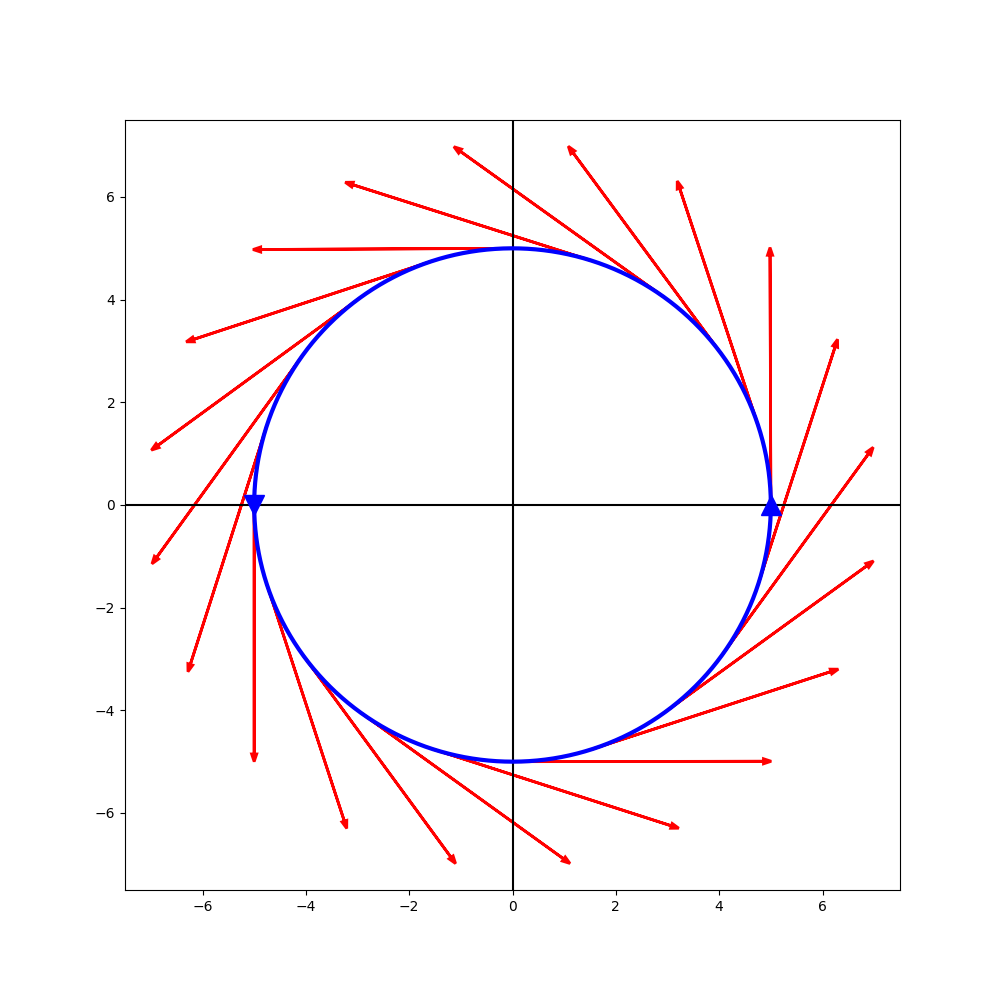
\includegraphics[width=1.0\textwidth]{hw5_figure_1}
% This file was created by matplotlib2tikz v0.6.13.
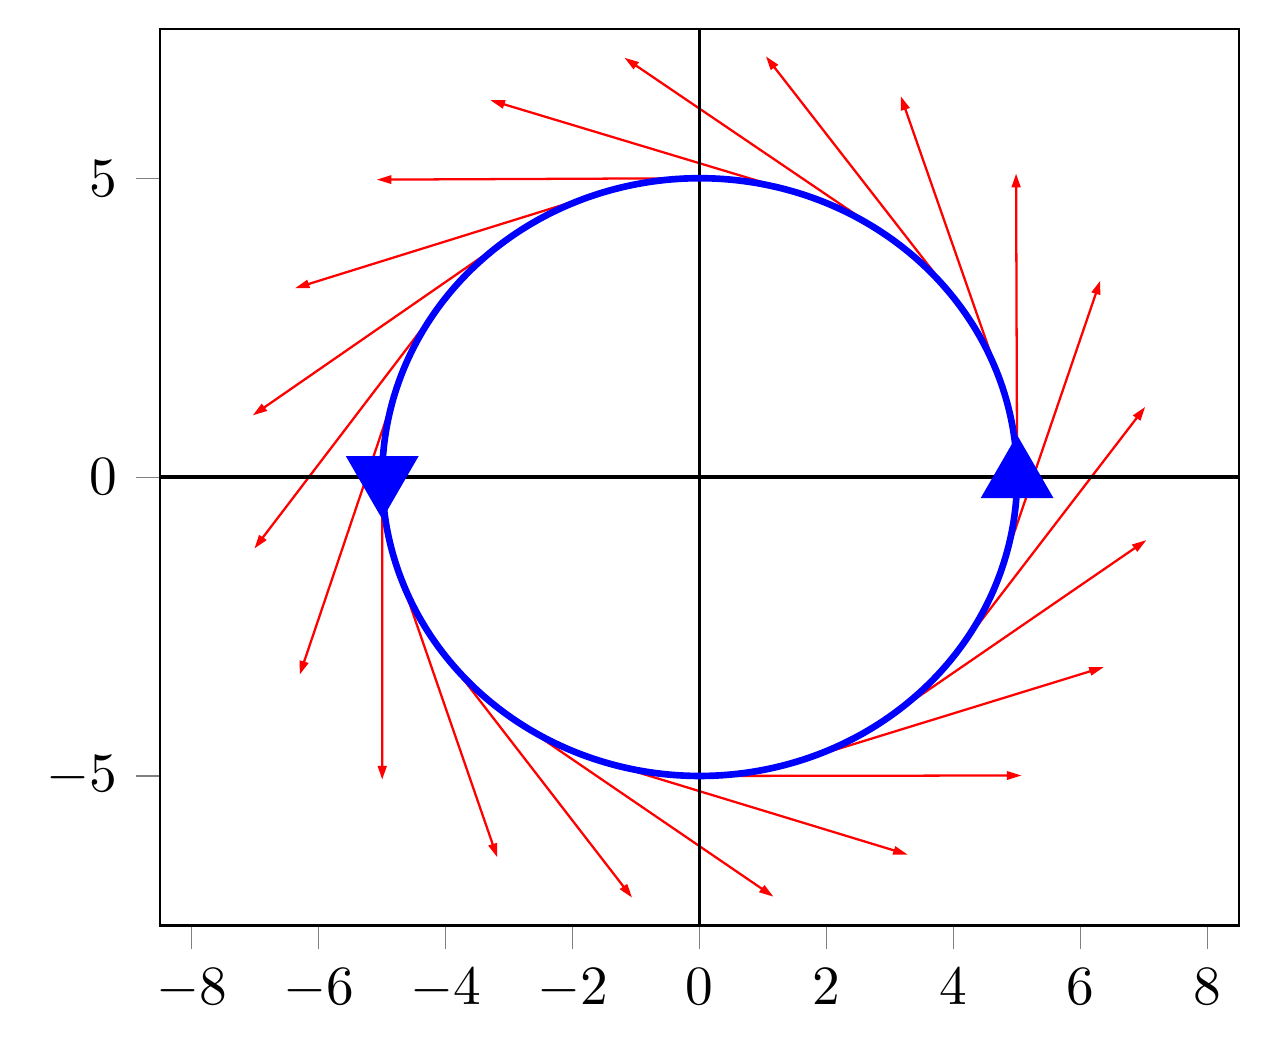
\begin{tikzpicture}[scale=2.0]

\begin{axis}[
xmin=-8.5, xmax=8.5,
ymin=-7.5, ymax=7.5,
tick align=outside,
tick pos=left,
x grid style={lightgray!92.026143790849673!black},
y grid style={lightgray!92.026143790849673!black}
]
\path [draw=red, fill=red] (axis cs:-5,-5)
--(axis cs:-5.05,-4.85)
--(axis cs:-5.0005,-4.85)
--(axis cs:-5.0005,-8.88178419700125e-16)
--(axis cs:-4.9995,-8.88178419700125e-16)
--(axis cs:-4.9995,-4.85)
--(axis cs:-4.95,-4.85)
--cycle;

\path [draw=red, fill=red] (axis cs:-3.20821615075728,-6.30137676464597)
--(axis cs:-3.30216152454263,-6.17419867398437)
--(axis cs:-3.25508903961138,-6.15888752894562)
--(axis cs:-4.7552719373474,-1.54673496497504)
--(axis cs:-4.75432097805586,-1.54642564891365)
--(axis cs:-3.25413808031984,-6.15857821288423)
--(axis cs:-3.2070655953886,-6.14326706784548)
--cycle;

\path [draw=red, fill=red] (axis cs:-1.10176591566475,-6.9847055676728)
--(axis cs:-1.23044236786156,-6.89282319368278)
--(axis cs:-1.19041433401904,-6.86370264240534)
--(axis cs:-4.04364006524294,-2.94176397298663)
--(axis cs:-4.04283141809461,-2.94117567902143)
--(axis cs:-1.1896056868707,-6.86311434844014)
--(axis cs:-1.14957765302818,-6.8339937971627)
--cycle;

\path [draw=red, fill=red] (axis cs:1.11274708154963,-6.98296455185781)
--(axis cs:0.961960319696975,-6.93538984797023)
--(axis cs:0.991017896175,-6.89531607538486)
--(axis cs:-2.93540224602761,-4.04826060228539)
--(axis cs:-2.93481522428058,-4.04745103112205)
--(axis cs:0.991604917922031,-6.89450650422152)
--(axis cs:1.02066249440006,-6.85443273163615)
--cycle;

\path [draw=red, fill=red] (axis cs:3.21812026833274,-6.29632447849902)
--(axis cs:3.06001257607944,-6.29772363908069)
--(axis cs:3.07524968691976,-6.25062713758387)
--(axis cs:-1.53925601529365,-4.75769809565322)
--(axis cs:-1.53894819487263,-4.75674665117854)
--(axis cs:3.07555750734078,-6.24967569310919)
--(axis cs:3.0907946181811,-6.20257919161237)
--cycle;

\path [draw=red, fill=red] (axis cs:5.00785565938091,-4.99213197890506)
--(axis cs:4.857934463209,-5.04236777230363)
--(axis cs:4.85785663099064,-4.99286783349412)
--(axis cs:0.00786262642194657,-5.0004938185249)
--(axis cs:0.00786105405389925,-4.99949381976107)
--(axis cs:4.8578550586226,-4.99186783473029)
--(axis cs:4.85777722640424,-4.94236789592077)
--cycle;

\path [draw=red, fill=red] (axis cs:6.30641347162941,-3.1983041013717)
--(axis cs:6.17938325488569,-3.29244932979057)
--(axis cs:6.16399811350291,-3.24540097780422)
--(axis cs:1.55421009059737,-4.75283402237921)
--(axis cs:1.55389927966034,-4.75188355062191)
--(axis cs:6.16368730256588,-3.24445050604692)
--(axis cs:6.14830216118311,-3.19740215406056)
--cycle;

\path [draw=red, fill=red] (axis cs:6.98642931490123,-1.09078202583684)
--(axis cs:6.89474938123548,-1.21960279187649)
--(axis cs:6.86556592715461,-1.17962059573984)
--(axis cs:2.94811842689665,-4.03900953093607)
--(axis cs:2.94752886216774,-4.038201809802)
--(axis cs:6.86497636242571,-1.17881287460577)
--(axis cs:6.83579290834484,-1.13883067846911)
--cycle;

\path [draw=red, fill=red] (axis cs:6.98120627176066,1.12372549634226)
--(axis cs:6.9338687189699,0.972864115943626)
--(axis cs:6.89374930671779,1.00185864578195)
--(axis cs:4.05287113063986,-2.92903326174797)
--(axis cs:4.05206063746305,-2.92844751367043)
--(axis cs:6.89293881354098,1.00244439385949)
--(axis cs:6.85281940128887,1.03143892369781)
--cycle;

\path [draw=red, fill=red] (axis cs:6.29125662567955,3.22801642961171)
--(axis cs:6.29290438801499,3.06991113280201)
--(axis cs:6.2457839863913,3.08507417177254)
--(axis cs:4.7601124912984,-1.53177326004372)
--(axis cs:4.75916056399287,-1.53146693602412)
--(axis cs:6.24483205908577,3.08538049579215)
--(axis cs:6.19771165746208,3.10054353476268)
--cycle;

\path [draw=red, fill=red] (axis cs:4.98425161554855,5.01569893762591)
--(axis cs:5.03472307814558,4.86585691593868)
--(axis cs:4.98522332290737,4.8657012516944)
--(axis cs:5.00047527411489,0.0157252334047842)
--(axis cs:4.99947527905957,0.0157220886725762)
--(axis cs:4.98422332785205,4.86569810696219)
--(axis cs:4.93472357261384,4.86554244271791)
--cycle;

\path [draw=red, fill=red] (axis cs:3.18838414468199,6.31143458699688)
--(axis cs:3.28272899497511,6.18455255823327)
--(axis cs:3.2357048922533,6.16909345854381)
--(axis cs:4.75038435677602,1.56168137367956)
--(axis cs:4.74943437490285,1.56136906863533)
--(axis cs:3.23475491038013,6.16878115349958)
--(axis cs:3.18773080765832,6.15332205381012)
--cycle;

\path [draw=red, fill=red] (axis cs:1.07979543922183,6.98813578928141)
--(axis cs:1.20876020061524,6.89665852260416)
--(axis cs:1.16882394103415,6.86741223787137)
--(axis cs:4.03436901081305,2.95446559204729)
--(axis cs:4.0335622176902,2.95387475801229)
--(axis cs:1.1680171479113,6.86682140383636)
--(axis cs:1.12808088833021,6.83757511910356)
--cycle;

\path [draw=red, fill=red] (axis cs:-1.13470113290025,6.9794307317284)
--(axis cs:-0.983765506936679,6.93233044706913)
--(axis cs:-1.01269691845088,6.89216549433921)
--(axis cs:2.92265703589402,4.05747163890756)
--(axis cs:2.92207256293414,4.0566602257211)
--(axis cs:-1.01328139141076,6.89135408115275)
--(axis cs:-1.04221280292496,6.85118912842284)
--cycle;

\path [draw=red, fill=red] (axis cs:-3.23790461012749,6.28617321871703)
--(axis cs:-3.07980209965187,6.28806957873241)
--(axis cs:-3.09489102926439,6.24092539347962)
--(axis cs:1.5242867177252,4.7625151183137)
--(axis cs:1.52398189086434,4.76156271053081)
--(axis cs:-3.09519585612525,6.23997298569674)
--(axis cs:-3.11028478573777,6.19282880044396)
--cycle;

\path [draw=red, fill=red] (axis cs:-5.02352981534373,4.97635892941341)
--(axis cs:-4.87376733860202,5.02706593642615)
--(axis cs:-4.87353384271667,4.97756648713961)
--(axis cs:-0.0235878015094535,5.00044436681581)
--(axis cs:-0.02358308442086,4.99944437794133)
--(axis cs:-4.87352912562807,4.97656649826513)
--(axis cs:-4.87329562974272,4.92706704897858)
--cycle;

\path [draw=red, fill=red] (axis cs:-6.31644009833446,3.17845630521368)
--(axis cs:-6.18970657124684,3.27300054412823)
--(axis cs:-6.17417355147089,3.22600080693067)
--(axis cs:-1.56914879575005,4.74792294659425)
--(axis cs:-1.56883499737073,4.74697345695389)
--(axis cs:-6.17385975309158,3.22505131729031)
--(axis cs:-6.15832673331563,3.17805158009275)
--cycle;

\path [draw=red, fill=red] (axis cs:-6.98982498659435,1.06880618298234)
--(axis cs:-6.89855061306876,1.19791462088441)
--(axis cs:-6.86924156999088,1.158024396595)
--(axis cs:-2.96080545274618,4.02971851634683)
--(axis cs:-2.96021335086582,4.02891265322987)
--(axis cs:-6.86864946811052,1.15721853347805)
--(axis cs:-6.83934042503264,1.11732830918864)
--cycle;

\path [draw=red, fill=red] (axis cs:-6.9776379361508,-1.14567396408806)
--(axis cs:-6.93077503607105,-0.994664465724162)
--(axis cs:-6.89056464216487,-1.02353268738587)
--(axis cs:-4.06206211571444,2.91627358422997)
--(axis cs:-4.06124978452442,2.91569038783277)
--(axis cs:-6.88975231097484,-1.02411588378308)
--(axis cs:-6.84954191706866,-1.05298410544479)
--cycle;

\path [draw=red, fill=red] (axis cs:-6.28107427017937,-3.2477847854331)
--(axis cs:-6.28321922318624,-3.08968545217518)
--(axis cs:-6.23605137086096,-3.10470023512467)
--(axis cs:-4.76490597075901,1.51679640684737)
--(axis cs:-4.76395308485345,1.5164930778989)
--(axis cs:-6.23509848495539,-3.10500356407315)
--(axis cs:-6.18793063263011,-3.12001834702264)
--cycle;

\addplot [semithick, black, forget plot]
table {%
-10 0
10 0
};
\addplot [semithick, black, forget plot]
table {%
0 -10
0 10
};
\addplot [very thick, blue, forget plot]
table {%
-5 -6.12323399573677e-16
-4.99990110659342 -0.0314471665803392
-4.99960443028563 -0.0628930891937056
-4.99910998281237 -0.0943365239223355
-4.99841778373267 -0.125776226946879
-4.99752786042811 -0.157210954595603
-4.9964402481017 -0.188639463393585
-4.99515498977652 -0.22006051011191
-4.993672136294 -0.251472851816832
-4.99199174631192 -0.282875245918963
-4.99011388630206 -0.314266450222411
-4.98803863054761 -0.345645222973924
-4.98576606114023 -0.377010322912009
-4.98329626797676 -0.408360509316034
-4.98062934875571 -0.439694542055307
-4.97776540897337 -0.471011181638131
-4.97470456191964 -0.50230918926084
-4.97144692867356 -0.533587326856794
-4.96799263809851 -0.564844357145364
-4.96434182683712 -0.596079043680866
-4.96049463930584 -0.627290150901482
-4.95645122768928 -0.658476444178119
-4.95221175193412 -0.689636689863269
-4.94777637974286 -0.720769655339792
-4.94314528656711 -0.751874109069684
-4.93831865560072 -0.782948820642789
-4.93329667777246 -0.813992560825472
-4.92807955173854 -0.845004101609246
-4.92266748387471 -0.875982216259345
-4.91706068826809 -0.906925679363255
-4.91125938670874 -0.937833266879185
-4.90526380868084 -0.968703756184488
-4.89907419135365 -0.999535926124022
-4.8926907795721 -1.03032855705846
-4.88611382584713 -1.06108043091254
-4.87934359034568 -1.09179033122323
-4.87238034088042 -1.12245704318786
-4.86522435289912 -1.1530793537122
-4.8578759094738 -1.1836560514584
-4.8503353012895 -1.21418592689294
-4.8426028266328 -1.24466777233446
-4.83467879137999 -1.27510038200155
-4.82656350898502 -1.30548255206044
-4.81825730046704 -1.33581308067261
-4.80976049439777 -1.36609076804233
-4.80107342688845 -1.39631441646415
-4.79219644157654 -1.42648283037025
-4.78312988961219 -1.45659481637774
-4.77387412964427 -1.48664918333586
-4.76442952780623 -1.51664474237313
-4.75479645770163 -1.54658030694435
-4.74497530038929 -1.57645469287751
-4.73496644436832 -1.60626671842072
-4.72477028556264 -1.63601520428886
-4.71438722730542 -1.66569897371029
-4.70381768032305 -1.69531685247338
-4.69306206271895 -1.72486766897295
-4.68212079995696 -1.75435025425665
-4.6709943248446 -1.78376344207116
-4.65968307751587 -1.81310606890834
-4.64818750541389 -1.84237697405125
-4.63650806327316 -1.8715749996201
-4.62464521310163 -1.90069899061798
-4.61259942416234 -1.92974779497664
-4.60037117295496 -1.95872026360199
-4.58796094319683 -1.98761525041957
-4.57536922580393 -2.01643161241991
-4.56259651887138 -2.04516820970373
-4.54964332765378 -2.07382390552703
-4.53651016454522 -2.10239756634607
-4.52319754905899 -2.13088806186218
-4.50970600780705 -2.15929426506649
-4.49603607447918 -2.18761505228452
-4.48218828982191 -2.21584930322063
-4.46816320161706 -2.24399590100231
-4.45396136466014 -2.27205373222439
-4.43958334073836 -2.30002168699306
-4.42502969860844 -2.32789865896979
-4.41030101397406 -2.35568354541509
-4.39539786946314 -2.38337524723214
-4.38032085460479 -2.41097266901024
-4.36507056580594 -2.43847471906817
-4.3496476063278 -2.46588030949737
-4.33405258626196 -2.49318835620496
-4.3182861225063 -2.52039777895662
-4.30234883874054 -2.54750750141937
-4.28624136540158 -2.57451645120406
-4.2699643396586 -2.6014235599079
-4.25351840538781 -2.6282277631566
-4.23690421314698 -2.6549280006466
-4.22012242014975 -2.68152321618691
-4.20317369023959 -2.70801235774095
-4.18605869386355 -2.73439437746814
-4.16877810804576 -2.76066823176535
-4.1513326163606 -2.78683288130821
-4.13372290890573 -2.81288729109218
-4.11594968227473 -2.83883043047354
-4.09801363952956 -2.8646612732101
-4.07991549017277 -2.89037879750185
-4.06165595011943 -2.91598198603137
-4.04323574166877 -2.94146982600403
-4.02465559347567 -2.9668413091881
-4.00591624052179 -2.99209543195463
-3.98701842408649 -3.01723119531713
-3.96796289171757 -3.04224760497109
-3.94875039720163 -3.06714367133331
-3.92938170053427 -3.09191840958108
-3.90985756789007 -3.11657083969108
-3.8901787715922 -3.14109998647821
-3.87034609008195 -3.16550487963411
-3.85036030788791 -3.18978455376556
-3.83022221559489 -3.2139380484327
-3.80993260981272 -3.23796440818697
-3.7894922931447 -3.26186268260896
-3.76890207415585 -3.28563192634594
-3.74816276734091 -3.30927119914934
-3.72727519309218 -3.33277956591186
-3.706240177667 -3.35615609670451
-3.68505855315511 -3.3793998668134
-3.6637311574457 -3.40250995677626
-3.6422588341943 -3.42548545241891
-3.6206424327894 -3.44832544489131
-3.59888280831882 -3.47102903070361
-3.57698082153591 -3.49359531176184
-3.55493733882551 -3.51602339540342
-3.53275323216966 -3.53831239443252
-3.51042937911311 -3.56046142715513
-3.48796666272861 -3.58246961741392
-3.46536597158198 -3.60433609462293
-3.44262819969696 -3.62605999380199
-3.41975424651983 -3.64764045561094
-3.39674501688385 -3.66907662638364
-3.37360142097346 -3.69036765816169
-3.35032437428829 -3.71151270872805
-3.3269147976069 -3.73251094164026
-3.30337361695041 -3.75336152626362
-3.27970176354584 -3.77406363780399
-3.25590017378928 -3.79461645734045
-3.23196978920885 -3.81501917185764
-3.20791155642744 -3.83527097427799
-3.1837264271253 -3.85537106349362
-3.15941535800236 -3.87531864439801
-3.13497931074039 -3.89511292791746
-3.11041925196498 -3.91475313104232
-3.08573615320728 -3.93423847685795
-3.06093099086557 -3.95356819457547
-3.03600474616666 -3.97274151956222
-3.01095840512705 -3.99175769337203
-2.98579295851393 -4.01061596377522
-2.960509401806 -4.02931558478835
-2.93510873515409 -4.04785581670372
-2.90959196334158 -4.06623592611867
-2.88396009574465 -4.08445518596453
-2.85821414629239 -4.10251287553544
-2.83235513342667 -4.12040828051682
-2.80638408006183 -4.13814069301366
-2.78030201354424 -4.15570941157847
-2.75410996561167 -4.17311374123909
-2.72780897235246 -4.19035299352613
-2.70140007416453 -4.20742648650025
-2.67488431571426 -4.22433354477909
-2.6482627458951 -4.24107349956401
-2.62153641778616 -4.25764568866656
-2.59470638861048 -4.27404945653463
-2.56777371969326 -4.29028415427844
-2.54073947641985 -4.30634913969615
-2.51360472819361 -4.32224377729932
-2.48637054839362 -4.33796743833801
-2.45903801433221 -4.35351950082564
-2.43160820721233 -4.36889934956364
-2.40408221208482 -4.38410637616577
-2.37646111780545 -4.39913997908215
-2.34874601699185 -4.4139995636231
-2.32093800598033 -4.42868454198265
-2.29303818478245 -4.44319433326178
-2.26504765704157 -4.45752836349142
-2.23696752998913 -4.47168606565514
-2.20879891440092 -4.48566687971157
-2.18054292455305 -4.49947025261659
-2.15220067817799 -4.51309563834517
-2.12377329642024 -4.52654249791298
-2.09526190379205 -4.53981029939773
-2.06666762812892 -4.55289851796018
-2.03799160054498 -4.56580663586492
-2.00923495538826 -4.57853414250085
-1.98039883019578 -4.59108053440137
-1.95148436564863 -4.60344531526432
-1.92249270552675 -4.61562799597156
-1.89342499666375 -4.62762809460839
-1.86428238890154 -4.63944513648255
-1.83506603504483 -4.65107865414302
-1.80577709081551 -4.66252818739854
-1.77641671480697 -4.67379328333576
-1.74698606843825 -4.68487349633719
-1.71748631590812 -4.69576838809884
-1.68791862414896 -4.70647752764752
-1.65828416278069 -4.71700049135791
-1.62858410406445 -4.72733686296932
-1.59881962285623 -4.73748623360215
-1.56899189656039 -4.74744820177407
-1.53910210508314 -4.75722237341588
-1.50915143078578 -4.76680836188715
-1.47914105843801 -4.77620578799143
-1.44907217517101 -4.78541427999135
-1.41894597043048 -4.79443347362325
-1.38876363592965 -4.80326301211161
-1.35852636560206 -4.81190254618317
-1.32823535555438 -4.82035173408075
-1.29789180401908 -4.82861024157677
-1.26749691130702 -4.83667774198645
-1.23705187976001 -4.84455391618075
-1.2065579137032 -4.85223845259898
-1.17601621939745 -4.85973104726117
-1.14542800499165 -4.86703140378001
-1.11479448047489 -4.87413923337267
-1.0841168576286 -4.88105425487215
-1.05339634997863 -4.88777619473843
-1.02263417274725 -4.89430478706931
-0.991831542805065 -4.90063977361088
-0.960989678622865 -4.9067809037678
-0.93010980022346 -4.91272793461314
-0.899193129133399 -4.91848063089805
-0.868240888334652 -4.92403876506104
-0.837254302216231 -4.92940211723698
-0.806234596525762 -4.9345704752658
-0.775182998320989 -4.93954363470089
-0.744100735921245 -4.94432139881718
-0.712989038858855 -4.94890357861892
-0.681849137830499 -4.95328999284716
-0.650682264648538 -4.95748046798692
-0.619489652192275 -4.96147483827407
-0.588272534359193 -4.96527294570184
-0.557032146016142 -4.96887464002712
-0.525769722950492 -4.97227977877639
-0.494486501821249 -4.97548822725133
-0.463183720110137 -4.97849985853419
-0.431862616072642 -4.98131455349277
-0.400524428689036 -4.98393220078517
-0.36917039761536 -4.98635269686416
-0.337801763134392 -4.98857594598131
-0.306419766106581 -4.99060186019073
-0.275025647920965 -4.99243035935261
-0.243620650446061 -4.99406137113635
-0.212206015980742 -4.99549483102341
-0.180782987205095 -4.9967306823099
-0.149352807131266 -4.99776887610882
-0.117916719054285 -4.99860937135194
-0.0864759665028868 -4.9992521347915
-0.0550317931903235 -4.99969714100147
-0.0235854429651605 -4.99994437237857
0.00786184023792268 -4.99999381914299
0.0393088124473406 -4.99984547933873
0.0707542297038099 -4.99949935883374
0.102196848109558 -4.99895547131963
0.133635423877524 -4.99821383831115
0.165068713380568 -4.99727448914535
0.196495473200656 -4.9961374609804
0.227914460178056 -4.99480279879414
0.259324431460505 -4.99327055538228
0.290724144552378 -4.99154079135634
0.322112357363841 -4.98961357514122
0.353487828259973 -4.9874889829725
0.384849316109897 -4.98516709889345
0.416195580335864 -4.98264801475168
0.447525380962333 -4.97993183019552
0.478837478665019 -4.97701865267006
0.510130634819921 -4.97390859741293
0.541403611552309 -4.9706017874497
0.572655171785704 -4.96709835358905
0.603884079290805 -4.9633984344176
0.635089098734393 -4.95950217629438
0.666268995728198 -4.9554097333451
0.697422536877727 -4.95112126745599
0.728548489831057 -4.94663694826747
0.759645623327578 -4.94195695316736
0.790712707246704 -4.93708146728394
0.82174851265653 -4.93201068347857
0.852751811862448 -4.92674480233808
0.883721378455707 -4.92128403216684
0.914655987361934 -4.91562858897852
0.945554414889581 -4.90977869648753
0.97641543877835 -4.9037345861002
1.00723783824753 -4.89749649690558
1.03802039404428 -4.89106467566604
1.06876188849188 -4.88443937680746
1.09946110553789 -4.87762086240919
1.13011683080225 -4.87060940219368
1.16072785162531 -4.8634052735158
1.19129295711582 -4.85600876135188
1.22181093819883 -4.84842015828844
1.25228058766349 -4.84063976451059
1.28270070021082 -4.83266788779021
1.31307007250141 -4.82450484347369
1.34338750320297 -4.81615095446956
1.37365179303791 -4.80760655123563
1.40386174483075 -4.79887197176595
1.43401616355545 -4.78994756157744
1.46411385638275 -4.78083367369625
1.4941536327273 -4.77153066864374
1.52413430429477 -4.76203891442226
1.55405468512886 -4.75235878650056
1.58391359165821 -4.74249066779898
1.61370984274325 -4.73243494867426
1.64344225972284 -4.72219202690414
1.67310966646101 -4.71176230767159
1.70271088939337 -4.70114620354879
1.73224475757362 -4.69034413448083
1.76171010271982 -4.67935652776906
1.79110575926064 -4.66818381805423
1.82043056438142 -4.65682644729927
1.84968335807022 -4.64528486477181
1.87886298316366 -4.63355952702643
1.90796828539274 -4.62165089788654
1.93699811342847 -4.60955944842613
1.96595131892739 -4.59728565695103
1.99482675657708 -4.58483000898007
2.02362328414137 -4.57219299722583
2.05233976250557 -4.55937512157517
2.08097505572154 -4.54637688906944
2.1095280310526 -4.53319881388445
2.13799755901835 -4.51984141731008
2.16638251343934 -4.50630522772972
2.19468177148165 -4.49259078059934
2.22289421370126 -4.47869861842628
2.25101872408837 -4.46462929074784
2.27905419011151 -4.45038335410953
2.30699950276158 -4.43596137204302
2.33485355659574 -4.42136391504389
2.36261524978106 -4.40659156054904
2.39028348413818 -4.39164489291384
2.41785716518472 -4.37652450338906
2.44533520217858 -4.36123099009743
2.47271650816109 -4.34576495800999
2.5 -4.33012701892219
2.52718459843232 -4.31431779142966
2.55426922810704 -4.29833790090373
2.58125281762764 -4.28218797946673
2.60813429959449 -4.26586866596696
2.63491261064705 -4.24938060595343
2.66158669150596 -4.2327244516503
2.68815548701494 -4.21590086193111
2.7146179461825 -4.1989105022927
2.74097302222355 -4.18175404482888
2.76721967260079 -4.16443216820387
2.79335685906596 -4.14694555762541
2.81938354770089 -4.12929490481772
2.84529870895842 -4.11148090799405
2.87110131770312 -4.09350427182914
2.89679035325183 -4.07536570743131
2.92236479941407 -4.05706593231433
2.9478236445322 -4.03860567036903
2.97316588152143 -4.0199856518347
2.99839050790972 -4.00120661327016
3.02349652587738 -3.98226929752464
3.04848294229653 -3.96317445370842
3.07334876877046 -3.94392283716316
3.09809302167264 -3.92451520943202
3.12271472218569 -3.90495233822959
3.14721289634008 -3.88523499741144
3.17158657505264 -3.86536396694359
3.19583479416492 -3.84534003287158
3.21995659448134 -3.82516398728945
3.24395102180709 -3.80483662830834
3.2678171269859 -3.78435876002496
3.29155396593759 -3.76373119248977
3.31516059969543 -3.74295474167495
3.33863609444324 -3.72203022944209
3.36197952155236 -3.70095848350972
3.38518995761838 -3.67974033742052
3.40826648449766 -3.65837663050839
3.43120818934367 -3.63686820786524
3.45401416464305 -3.61521592030755
3.47668350825159 -3.59342062434269
3.49921532342983 -3.57148318213511
3.52160871887858 -3.54940446147214
3.54386280877419 -3.52718533572977
3.56597671280355 -3.50482668383799
3.58794955619894 -3.48232939024611
3.60978046977262 -3.45969434488773
3.63146858995124 -3.43692244314555
3.65301305880994 -3.41401458581595
3.67441302410638 -3.39097167907333
3.69566763931436 -3.36779463443433
3.71677606365735 -3.3444843687217
3.73773746214177 -3.32104180402807
3.75855100558997 -3.29746786767948
3.77921587067306 -3.27376349219868
3.79973123994349 -3.24992961526823
3.82009630186735 -3.22596717969347
3.8403102508565 -3.20187713336513
3.86037228730043 -3.17766042922192
3.88028161759789 -3.15331802521279
3.90003745418829 -3.12885088425903
3.91963901558283 -3.10425997421622
3.93908552639543 -3.0795462678359
3.95837621737343 -3.05471074272711
3.97751032542795 -3.02975438131774
3.99648709366415 -3.00467817081562
4.01530577141113 -2.97948310316949
4.03396561425162 -2.95417017502979
4.05246588405146 -2.9287403877092
4.07080584898876 -2.90319474714303
4.08898478358289 -2.87753426384945
4.10700196872313 -2.85175995288951
4.12485669169715 -2.82587283382696
4.14254824621921 -2.79987393068798
4.16007593245807 -2.77376427192059
4.17743905706468 -2.74754489035403
4.19463693319964 -2.7212168231579
4.21166888056031 -2.69478111180108
4.22853422540778 -2.66823880201061
4.24523230059349 -2.64159094373026
4.26176244558562 -2.61483859107901
4.27812400649523 -2.58798280230939
4.29431633610213 -2.56102463976557
4.31033879388046 -2.53396516984136
4.32619074602404 -2.50680546293803
4.34187156547146 -2.47954659342195
4.35738063193086 -2.4521896395821
4.37271733190447 -2.42473568358744
4.38788105871289 -2.39718581144405
4.40287121251907 -2.36954111295222
4.41768720035208 -2.3418026816633
4.43232843613049 -2.3139716148365
4.44679434068565 -2.2860490133954
4.46108434178452 -2.25803598188448
4.47519787415234 -2.22993362842538
4.489134379495 -2.2017430646731
4.50289330652109 -2.17346540577198
4.51647411096376 -2.14510177031163
4.5298762556022 -2.11665328028267
4.54309921028291 -2.08812106103233
4.55614245194068 -2.05950624121996
4.56900546461927 -2.03080995277236
4.58168773949182 -2.00203333083902
4.59418877488098 -1.9731775137472
4.60650807627877 -1.94424364295694
4.61864515636611 -1.91523286301584
4.63059953503213 -1.88614632151385
4.64237073939313 -1.85698516903784
4.65395830381131 -1.8277505591261
4.66536176991319 -1.79844364822268
4.67658068660771 -1.76906559563169
4.68761461010414 -1.73961756347142
4.69846310392954 -1.71010071662834
4.70912573894612 -1.68051622271108
4.71960209336816 -1.65086525200418
4.72989175277871 -1.62114897742186
4.73999431014598 -1.59136857446154
4.74990936583943 -1.56152522115745
4.75963652764563 -1.53162009803392
4.7691754107837 -1.50165438805875
4.77852563792058 -1.47162927659641
4.78768683918595 -1.44154595136111
4.79665865218685 -1.41140560236986
4.80544072202201 -1.38120942189537
4.81403270129592 -1.35095860441891
4.82243425013254 -1.32065434658303
4.83064503618874 -1.29029784714425
4.83866473466749 -1.25989030692563
4.84649302833068 -1.22943292876925
4.85412960751164 -1.19892691748868
4.86157417012744 -1.16837347982126
4.86882642169083 -1.13777382438041
4.87588607532186 -1.1071291616078
4.88275285175925 -1.07644070372545
4.88942647937142 -1.04570966468784
4.89590669416729 -1.01493726013381
4.90219323980663 -0.984124707338527
4.90828586761029 -0.953273225165323
4.91418433656997 -0.922384034017462
4.91988841335781 -0.89145835578988
4.92539787233556 -0.860497413820846
4.93071249556356 -0.829502432843568
4.93583207280933 -0.798474638937748
4.9407564015559 -0.767415259481082
4.94548528700981 -0.736325523100707
4.95001854210882 -0.705206659624598
4.95435598752932 -0.674059900032923
4.9584974516934 -0.642886476409345
4.96244277077568 -0.611687621892286
4.96619178870971 -0.580464570626151
4.96974435719426 -0.5492185577125
4.97310033569907 -0.517950819161197
4.9762595914705 -0.486662591841514
4.9792219995367 -0.455355113433205
4.98198744271263 -0.424029622377547
4.98455581160466 -0.392687357828349
4.98692700461488 -0.361329559602936
4.98910092794515 -0.329957468133104
4.9910774956008 -0.298572324416051
4.99285662939403 -0.267175369965289
4.99443825894699 -0.23576784676153
4.99582232169459 -0.204350997203558
4.99700876288696 -0.172926064059087
4.99799753559161 -0.141494290415591
4.9987886006953 -0.110056919631138
4.99938192690559 -0.0786151952852057
4.99977749075205 -0.0471703611294846
4.99997527658723 -0.0157236610386828
4.99997527658723 0.0157236610386806
4.99977749075205 0.0471703611294824
4.99938192690559 0.0786151952852034
4.9987886006953 0.110056919631136
4.99799753559161 0.141494290415589
4.99700876288696 0.172926064059084
4.99582232169459 0.204350997203558
4.99443825894699 0.235767846761528
4.99285662939403 0.267175369965287
4.9910774956008 0.298572324416049
4.98910092794515 0.329957468133102
4.98692700461488 0.361329559602934
4.98455581160466 0.392687357828347
4.98198744271263 0.424029622377545
4.9792219995367 0.455355113433203
4.9762595914705 0.486662591841512
4.97310033569907 0.517950819161195
4.96974435719426 0.549218557712498
4.96619178870971 0.580464570626149
4.96244277077568 0.611687621892286
4.9584974516934 0.642886476409343
4.95435598752932 0.674059900032921
4.95001854210882 0.705206659624596
4.94548528700981 0.736325523100705
4.9407564015559 0.76741525948108
4.93583207280933 0.798474638937746
4.93071249556356 0.829502432843565
4.92539787233556 0.860497413820844
4.91988841335781 0.891458355789878
4.91418433656997 0.92238403401746
4.90828586761029 0.953273225165321
4.90219323980663 0.984124707338525
4.89590669416729 1.01493726013381
4.88942647937143 1.04570966468784
4.88275285175925 1.07644070372545
4.87588607532186 1.10712916160779
4.86882642169083 1.13777382438041
4.86157417012745 1.16837347982126
4.85412960751164 1.19892691748868
4.84649302833068 1.22943292876925
4.83866473466749 1.25989030692562
4.83064503618874 1.29029784714425
4.82243425013254 1.32065434658303
4.81403270129592 1.35095860441891
4.80544072202201 1.38120942189537
4.79665865218685 1.41140560236986
4.78768683918595 1.44154595136111
4.77852563792058 1.47162927659641
4.7691754107837 1.50165438805875
4.75963652764563 1.53162009803392
4.74990936583944 1.56152522115745
4.73999431014598 1.59136857446154
4.72989175277871 1.62114897742185
4.71960209336817 1.65086525200418
4.70912573894612 1.68051622271108
4.69846310392954 1.71010071662834
4.68761461010414 1.73961756347142
4.67658068660771 1.76906559563169
4.66536176991319 1.79844364822268
4.65395830381131 1.82775055912609
4.64237073939313 1.85698516903784
4.63059953503213 1.88614632151385
4.61864515636611 1.91523286301584
4.60650807627877 1.94424364295694
4.59418877488098 1.9731775137472
4.58168773949182 2.00203333083902
4.56900546461927 2.03080995277236
4.55614245194068 2.05950624121996
4.54309921028291 2.08812106103233
4.5298762556022 2.11665328028267
4.51647411096376 2.14510177031163
4.50289330652109 2.17346540577198
4.489134379495 2.2017430646731
4.47519787415234 2.22993362842538
4.46108434178452 2.25803598188447
4.44679434068565 2.28604901339539
4.43232843613049 2.31397161483649
4.41768720035208 2.3418026816633
4.40287121251907 2.36954111295221
4.38788105871289 2.39718581144405
4.37271733190447 2.42473568358744
4.35738063193086 2.4521896395821
4.34187156547146 2.47954659342195
4.32619074602404 2.50680546293803
4.31033879388046 2.53396516984136
4.29431633610213 2.56102463976557
4.27812400649523 2.58798280230939
4.26176244558562 2.61483859107901
4.24523230059349 2.64159094373026
4.22853422540778 2.66823880201061
4.21166888056031 2.69478111180108
4.19463693319964 2.72121682315789
4.17743905706468 2.74754489035403
4.16007593245807 2.77376427192058
4.14254824621921 2.79987393068797
4.12485669169715 2.82587283382696
4.10700196872313 2.85175995288951
4.08898478358289 2.87753426384945
4.07080584898876 2.90319474714303
4.05246588405146 2.9287403877092
4.03396561425162 2.95417017502979
4.01530577141113 2.97948310316949
3.99648709366415 3.00467817081561
3.97751032542795 3.02975438131774
3.95837621737343 3.05471074272711
3.93908552639544 3.0795462678359
3.91963901558283 3.10425997421622
3.90003745418829 3.12885088425903
3.88028161759789 3.15331802521279
3.86037228730043 3.17766042922192
3.8403102508565 3.20187713336513
3.82009630186735 3.22596717969347
3.79973123994349 3.24992961526823
3.77921587067306 3.27376349219867
3.75855100558997 3.29746786767948
3.73773746214177 3.32104180402807
3.71677606365735 3.3444843687217
3.69566763931436 3.36779463443433
3.67441302410638 3.39097167907333
3.65301305880994 3.41401458581594
3.63146858995124 3.43692244314555
3.60978046977262 3.45969434488773
3.58794955619894 3.48232939024611
3.56597671280355 3.50482668383799
3.54386280877419 3.52718533572977
3.52160871887858 3.54940446147214
3.49921532342983 3.5714831821351
3.47668350825159 3.59342062434269
3.45401416464306 3.61521592030755
3.43120818934367 3.63686820786524
3.40826648449767 3.65837663050839
3.38518995761838 3.67974033742052
3.36197952155236 3.70095848350972
3.33863609444324 3.72203022944209
3.31516059969543 3.74295474167495
3.29155396593759 3.76373119248977
3.2678171269859 3.78435876002496
3.24395102180709 3.80483662830834
3.21995659448134 3.82516398728945
3.19583479416493 3.84534003287158
3.17158657505264 3.86536396694359
3.14721289634008 3.88523499741144
3.1227147221857 3.90495233822959
3.09809302167264 3.92451520943202
3.07334876877046 3.94392283716316
3.04848294229653 3.96317445370842
3.02349652587738 3.98226929752464
2.99839050790972 4.00120661327016
2.97316588152144 4.0199856518347
2.9478236445322 4.03860567036903
2.92236479941408 4.05706593231433
2.89679035325184 4.07536570743131
2.87110131770312 4.09350427182914
2.84529870895842 4.11148090799405
2.81938354770089 4.12929490481772
2.79335685906596 4.14694555762541
2.76721967260079 4.16443216820387
2.74097302222355 4.18175404482888
2.7146179461825 4.1989105022927
2.68815548701494 4.21590086193111
2.66158669150596 4.2327244516503
2.63491261064705 4.24938060595343
2.60813429959449 4.26586866596696
2.58125281762765 4.28218797946673
2.55426922810704 4.29833790090373
2.52718459843233 4.31431779142965
2.5 4.33012701892219
2.47271650816109 4.34576495800999
2.44533520217859 4.36123099009743
2.41785716518472 4.37652450338906
2.39028348413818 4.39164489291384
2.36261524978106 4.40659156054904
2.33485355659574 4.42136391504389
2.30699950276159 4.43596137204302
2.27905419011151 4.45038335410953
2.25101872408837 4.46462929074784
2.22289421370127 4.47869861842628
2.19468177148165 4.49259078059934
2.16638251343935 4.50630522772972
2.13799755901835 4.51984141731008
2.1095280310526 4.53319881388445
2.08097505572154 4.54637688906944
2.05233976250557 4.55937512157517
2.02362328414137 4.57219299722583
1.99482675657708 4.58483000898007
1.9659513189274 4.59728565695103
1.93699811342847 4.60955944842613
1.90796828539275 4.62165089788654
1.87886298316366 4.63355952702642
1.84968335807022 4.64528486477181
1.82043056438142 4.65682644729927
1.79110575926064 4.66818381805423
1.76171010271982 4.67935652776906
1.73224475757362 4.69034413448083
1.70271088939337 4.70114620354879
1.67310966646101 4.71176230767159
1.64344225972285 4.72219202690414
1.61370984274325 4.73243494867426
1.58391359165822 4.74249066779898
1.55405468512886 4.75235878650056
1.52413430429477 4.76203891442226
1.4941536327273 4.77153066864374
1.46411385638276 4.78083367369625
1.43401616355545 4.78994756157744
1.40386174483075 4.79887197176595
1.37365179303792 4.80760655123563
1.34338750320297 4.81615095446956
1.31307007250141 4.82450484347369
1.28270070021083 4.83266788779021
1.2522805876635 4.84063976451059
1.22181093819884 4.84842015828844
1.19129295711583 4.85600876135188
1.16072785162531 4.8634052735158
1.13011683080225 4.87060940219368
1.09946110553789 4.87762086240919
1.06876188849188 4.88443937680746
1.03802039404428 4.89106467566604
1.00723783824753 4.89749649690558
0.976415438778352 4.9037345861002
0.945554414889581 4.90977869648753
0.914655987361936 4.91562858897852
0.883721378455709 4.92128403216684
0.852751811862451 4.92674480233808
0.821748512656531 4.93201068347857
0.790712707246707 4.93708146728394
0.759645623327579 4.94195695316736
0.728548489831061 4.94663694826747
0.697422536877729 4.95112126745599
0.666268995728202 4.9554097333451
0.635089098734395 4.95950217629438
0.603884079290805 4.9633984344176
0.572655171785707 4.96709835358905
0.541403611552309 4.9706017874497
0.510130634819923 4.97390859741293
0.47883747866502 4.97701865267006
0.447525380962336 4.97993183019552
0.416195580335865 4.98264801475168
0.3848493161099 4.98516709889345
0.353487828259974 4.9874889829725
0.322112357363844 4.98961357514122
0.290724144552381 4.99154079135634
0.259324431460509 4.99327055538228
0.227914460178058 4.99480279879414
0.196495473200656 4.9961374609804
0.16506871338057 4.99727448914535
0.133635423877524 4.99821383831115
0.10219684810956 4.99895547131963
0.070754229703811 4.99949935883374
0.0393088124473439 4.99984547933873
0.00786184023792379 4.99999381914299
-0.0235854429651572 4.99994437237857
-0.0550317931903223 4.99969714100147
-0.0864759665028835 4.9992521347915
-0.117916719054283 4.99860937135194
-0.149352807131262 4.99776887610882
-0.180782987205093 4.9967306823099
-0.212206015980742 4.99549483102341
-0.243620650446059 4.99406137113635
-0.275025647920965 4.99243035935261
-0.306419766106579 4.99060186019073
-0.337801763134391 4.98857594598131
-0.369170397615357 4.98635269686416
-0.400524428689035 4.98393220078517
-0.431862616072639 4.98131455349277
-0.463183720110135 4.97849985853419
-0.494486501821245 4.97548822725133
-0.52576972295049 4.97227977877639
-0.557032146016137 4.96887464002712
-0.588272534359191 4.96527294570184
-0.619489652192275 4.96147483827407
-0.650682264648536 4.95748046798692
-0.681849137830499 4.95328999284716
-0.712989038858852 4.94890357861892
-0.744100735921244 4.94432139881718
-0.775182998320986 4.93954363470089
-0.80623459652576 4.9345704752658
-0.837254302216228 4.92940211723698
-0.86824088833465 4.92403876506104
-0.899193129133396 4.91848063089805
-0.930109800223458 4.91272793461314
-0.96098967862286 4.9067809037678
-0.991831542805062 4.90063977361088
-1.02263417274725 4.89430478706931
-1.05339634997863 4.88777619473843
-1.0841168576286 4.88105425487215
-1.11479448047488 4.87413923337267
-1.14542800499165 4.86703140378001
-1.17601621939745 4.85973104726117
-1.2065579137032 4.85223845259898
-1.23705187976001 4.84455391618075
-1.26749691130702 4.83667774198645
-1.29789180401907 4.82861024157677
-1.32823535555438 4.82035173408075
-1.35852636560206 4.81190254618317
-1.38876363592965 4.80326301211161
-1.41894597043048 4.79443347362325
-1.449072175171 4.78541427999135
-1.47914105843801 4.77620578799143
-1.50915143078578 4.76680836188715
-1.53910210508314 4.75722237341588
-1.56899189656039 4.74744820177407
-1.59881962285623 4.73748623360215
-1.62858410406445 4.72733686296932
-1.65828416278069 4.71700049135791
-1.68791862414896 4.70647752764752
-1.71748631590811 4.69576838809884
-1.74698606843825 4.68487349633719
-1.77641671480697 4.67379328333576
-1.80577709081551 4.66252818739854
-1.83506603504482 4.65107865414302
-1.86428238890154 4.63944513648255
-1.89342499666375 4.62762809460839
-1.92249270552674 4.61562799597156
-1.95148436564862 4.60344531526432
-1.98039883019578 4.59108053440137
-2.00923495538825 4.57853414250085
-2.03799160054498 4.56580663586492
-2.06666762812892 4.55289851796018
-2.09526190379205 4.53981029939773
-2.12377329642023 4.52654249791299
-2.15220067817799 4.51309563834517
-2.18054292455305 4.49947025261659
-2.20879891440091 4.48566687971157
-2.23696752998913 4.47168606565514
-2.26504765704157 4.45752836349142
-2.29303818478245 4.44319433326178
-2.32093800598033 4.42868454198265
-2.34874601699185 4.4139995636231
-2.37646111780545 4.39913997908215
-2.40408221208482 4.38410637616577
-2.43160820721233 4.36889934956364
-2.45903801433221 4.35351950082564
-2.48637054839362 4.33796743833801
-2.51360472819361 4.32224377729933
-2.54073947641985 4.30634913969615
-2.56777371969326 4.29028415427844
-2.59470638861048 4.27404945653463
-2.62153641778616 4.25764568866656
-2.6482627458951 4.24107349956401
-2.67488431571426 4.22433354477909
-2.70140007416453 4.20742648650025
-2.72780897235246 4.19035299352613
-2.75410996561167 4.17311374123909
-2.78030201354423 4.15570941157847
-2.80638408006182 4.13814069301366
-2.83235513342667 4.12040828051682
-2.85821414629239 4.10251287553544
-2.88396009574465 4.08445518596453
-2.90959196334157 4.06623592611867
-2.93510873515409 4.04785581670372
-2.960509401806 4.02931558478835
-2.98579295851393 4.01061596377522
-3.01095840512704 3.99175769337203
-3.03600474616666 3.97274151956222
-3.06093099086557 3.95356819457547
-3.08573615320727 3.93423847685795
-3.11041925196498 3.91475313104232
-3.13497931074039 3.89511292791746
-3.15941535800236 3.87531864439801
-3.1837264271253 3.85537106349362
-3.20791155642744 3.83527097427799
-3.23196978920884 3.81501917185764
-3.25590017378928 3.79461645734045
-3.27970176354584 3.774063637804
-3.30337361695041 3.75336152626362
-3.32691479760689 3.73251094164026
-3.35032437428829 3.71151270872805
-3.37360142097346 3.6903676581617
-3.39674501688385 3.66907662638364
-3.41975424651983 3.64764045561094
-3.44262819969696 3.62605999380199
-3.46536597158198 3.60433609462293
-3.48796666272861 3.58246961741392
-3.51042937911311 3.56046142715513
-3.53275323216966 3.53831239443252
-3.55493733882551 3.51602339540342
-3.57698082153591 3.49359531176184
-3.59888280831882 3.47102903070361
-3.6206424327894 3.44832544489131
-3.6422588341943 3.42548545241891
-3.6637311574457 3.40250995677627
-3.6850585531551 3.3793998668134
-3.706240177667 3.35615609670452
-3.72727519309218 3.33277956591186
-3.74816276734091 3.30927119914934
-3.76890207415585 3.28563192634594
-3.7894922931447 3.26186268260896
-3.80993260981272 3.23796440818697
-3.83022221559489 3.2139380484327
-3.8503603078879 3.18978455376556
-3.87034609008195 3.16550487963411
-3.8901787715922 3.14109998647821
-3.90985756789006 3.11657083969108
-3.92938170053427 3.09191840958108
-3.94875039720163 3.06714367133331
-3.96796289171757 3.04224760497109
-3.98701842408649 3.01723119531713
-4.00591624052179 2.99209543195463
-4.02465559347567 2.9668413091881
-4.04323574166877 2.94146982600403
-4.06165595011943 2.91598198603137
-4.07991549017277 2.89037879750185
-4.09801363952956 2.8646612732101
-4.11594968227473 2.83883043047354
-4.13372290890573 2.81288729109219
-4.1513326163606 2.78683288130821
-4.16877810804576 2.76066823176535
-4.18605869386355 2.73439437746814
-4.20317369023959 2.70801235774095
-4.22012242014975 2.68152321618691
-4.23690421314698 2.6549280006466
-4.25351840538781 2.62822776315661
-4.2699643396586 2.6014235599079
-4.28624136540158 2.57451645120407
-4.30234883874054 2.54750750141937
-4.3182861225063 2.52039777895663
-4.33405258626196 2.49318835620496
-4.3496476063278 2.46588030949738
-4.36507056580594 2.43847471906817
-4.38032085460479 2.41097266901024
-4.39539786946314 2.38337524723214
-4.41030101397405 2.35568354541509
-4.42502969860844 2.32789865896979
-4.43958334073836 2.30002168699306
-4.45396136466014 2.27205373222439
-4.46816320161706 2.24399590100231
-4.48218828982191 2.21584930322063
-4.49603607447918 2.18761505228452
-4.50970600780705 2.15929426506649
-4.52319754905899 2.13088806186218
-4.53651016454522 2.10239756634608
-4.54964332765378 2.07382390552704
-4.56259651887138 2.04516820970373
-4.57536922580393 2.01643161241991
-4.58796094319683 1.98761525041957
-4.60037117295496 1.95872026360199
-4.61259942416234 1.92974779497664
-4.62464521310162 1.90069899061799
-4.63650806327316 1.8715749996201
-4.64818750541388 1.84237697405125
-4.65968307751587 1.81310606890834
-4.6709943248446 1.78376344207116
-4.68212079995696 1.75435025425665
-4.69306206271894 1.72486766897296
-4.70381768032305 1.69531685247338
-4.71438722730542 1.66569897371029
-4.72477028556264 1.63601520428886
-4.73496644436831 1.60626671842072
-4.74497530038929 1.57645469287751
-4.75479645770163 1.54658030694435
-4.76442952780623 1.51664474237314
-4.77387412964427 1.48664918333586
-4.78312988961219 1.45659481637774
-4.79219644157654 1.42648283037025
-4.80107342688845 1.39631441646415
-4.80976049439777 1.36609076804233
-4.81825730046704 1.33581308067261
-4.82656350898502 1.30548255206044
-4.83467879137999 1.27510038200156
-4.8426028266328 1.24466777233446
-4.8503353012895 1.21418592689294
-4.8578759094738 1.1836560514584
-4.86522435289912 1.1530793537122
-4.87238034088042 1.12245704318787
-4.87934359034568 1.09179033122323
-4.88611382584713 1.06108043091254
-4.8926907795721 1.03032855705846
-4.89907419135365 0.999535926124027
-4.90526380868084 0.96870375618449
-4.91125938670874 0.93783326687919
-4.91706068826809 0.906925679363258
-4.92266748387471 0.875982216259349
-4.92807955173854 0.845004101609248
-4.93329667777246 0.813992560825472
-4.93831865560072 0.782948820642791
-4.94314528656711 0.751874109069684
-4.94777637974286 0.720769655339795
-4.95221175193412 0.689636689863269
-4.95645122768928 0.658476444178122
-4.96049463930584 0.627290150901482
-4.96434182683712 0.596079043680871
-4.96799263809851 0.564844357145366
-4.97144692867356 0.533587326856799
-4.97470456191964 0.502309189260842
-4.97776540897337 0.471011181638136
-4.98062934875571 0.439694542055309
-4.98329626797676 0.408360509316034
-4.98576606114023 0.377010322912011
-4.98803863054761 0.345645222973924
-4.99011388630206 0.314266450222413
-4.99199174631192 0.282875245918963
-4.993672136294 0.251472851816835
-4.99515498977652 0.22006051011191
-4.9964402481017 0.18863946339359
-4.99752786042811 0.157210954595605
-4.99841778373267 0.125776226946884
-4.99910998281237 0.0943365239223378
-4.99960443028563 0.06289308919371
-4.99990110659342 0.0314471665803414
-5 6.12323399573677e-16
};
\addplot [semithick, blue, mark=triangle*, mark size=7, mark options={solid}, only marks, forget plot]
table {%
5 0
};
\addplot [semithick, blue, mark=triangle*, mark size=7, mark options={solid,rotate=180}, only marks, forget plot]
table {%
-5 0
};
\end{axis}

\end{tikzpicture}

\problem{(b)}
	Since the velocity field at each point on the curve is pointing in the direction of the curve, we expect the circulation to be positive.

\problem{(c)}
	Since the velocity field at each point on the curve is tangent to the curve, we expect the flux to be zero.
	
\problem{(d)}
	First note the parametaraization of our curve: $r(t) = [5\text{cos}(t), 5 \text{sin}(t)]^T$ for $0 \leq t \leq 2\pi$.
	Using our equation for circulation where $M(x,y) = -y$ and $N(x,y) = x$ we get
	\begin{align*}
		\text{circ} & = \int_{C}(Mdx + Ndy) \\
		& = \int_{0}^{2\pi} M\big(x(t),y(t)\big)\tfrac{dx}{dt} + N\big(x(t),y(t)\big) \tfrac{dy}{dt} dt \\
		& = \int_{0}^{2\pi} -5 \text{sin}(t)(-5\text{sin}(t)) + 5\text{cos}(t)(5\text{cos}(t)) dt \\
		& = \int_{0}^{2\pi} 25(\sin^2 t+\cos^2 t) dt \\
		& = 25\int_{0}^{2\pi} 1 dt \\
		& = 50\pi
	\end{align*}
	As expected the circulation is positive.\\
	
\problem{(e)}
	With the same parametariziation as above we calculate the flux as follows
	\begin{align*}
		\text{flux} & = \int_{C}(Mdy - Ndx) \\
		& = \int_{0}^{2\pi} M\big(x(t),y(t)\big)\tfrac{dy}{dt} - N\big(x(t),y(t)\big) \tfrac{dx}{dt} dt \\
		& = \int_{0}^{2\pi} -5 \text{sin}(t)(5\text{cos}(t)) - 5\text{cos}(t)(-5\text{sin}(t)) dt \\
		& = \int_{0}^{2\pi} 0 dt \\
		& = 0
	\end{align*}
	The flux is zero as expected.
	
\problem{(f)}
	We will now compute the circulation using Green's Theorem.
	\begin{align*}
		\text{circ} = \int_{C}(Mdx + Ndy) & = \iint_{R}\Big(\frac{\partial N}{\partial x} - \frac{\partial M}{\partial y}\Big) dA \\
		& = \iint_{R}\big(1 - (-1)\big) dA \\
		& = \iint_{R}2 dA \\
		& = 50 \pi
	\end{align*}
	As expected, Green's Theorem gives the same result as our line integral.
	
\problem{(g)}
	We will now compute the flux using Green's Theorem as before. However, this time we will need to change to polar coordinates via the following substitutions: \bigbreak
	\begin{align*}
		x &= r\cos \theta & y &= r\sin \theta \\
		dA &= r dr d\theta&& \\
		\text{where } 0 & \leq r \leq 5 & \text{and } 0 &\leq \theta \leq 2\pi
	\end{align*} \bigbreak
	We calculate flux like so
	\begin{align*}
		\text{flux} = \int_{C}(Mdy - Ndx) & = \iint_{R}\Big(\frac{\partial M}{\partial x} + \frac{\partial N}{\partial y}\Big) dA \\
		& = \iint_{R}-y + x dA \\
		& = \int_{0}^{2\pi} \int_{0}^{5} (-\sin \theta + cos \theta) r dr d\theta \\
		& = \int_{0}^{2\pi} (-\sin \theta + cos \theta)\int_{0}^{5} r dr d\theta \\
		& = \int_{0}^{2\pi} (-\sin \theta + cos \theta)\Bigg( \tfrac{1}{2}r^2 \Big\vert_{0}^{5}\Bigg) d\theta \\
		& = \int_{0}^{2\pi} (-\sin \theta + cos \theta)\tfrac{25}{2} d\theta \\
		& = \tfrac{25}{2} \Bigg( cos \theta + \sin(\theta)\Big\vert_{0}^{2\pi}\Bigg) \\
		& = 0
	\end{align*}
	As expected, Green's Theorem gives the same result as our line integral.
	
\end{document}
